\chapter{Experiments and Results}

This should most likely contain both the results from the classification task and the visualization task.

\textcolor{blue}{(8-10 pages) In this chapter you present your results from your work, coming from 
testing/validating/exploring the theory/research-questions by empirical studies. It can be structured by contributions, 
research questions, or studies done. Find what suits your thesis and results. Some also like to include the 
bibliography of the included papers with abstract and identified contributions towards the thesis. Do not use all of 
the headlines below, if it leads to the same point being said over and over. Find the approach that best makes your 
point.}

\section{Developer Tools}
\textcolor{blue}{Describe what system and tools we use for the experiments}


\section{Description of Experiment}
\textcolor{blue}{Describe how the experiment was conducted.}

To experiment with different solutions for sentiment analysis, a system testing platform and code base was developed. This testing system generates and trains different models based on input arguments as default values for algorithms and type of algorithm. The architecture and flow of this system is described as a part of section~\ref{sec:classifier_arch}.

The testing system can take in a set of parameters to use for an algorithm, like pre-processor methods, whether or not to use inverse document frequency (IDF) or stop words and so on, or a grid search flag can be set. If the grid search option is activated, a model is generated with the best possible parameters set for the given algorithm. The grid search is conducted using cross validation, and the set of parameters to search across. The parameter search space is reflected in table~\ref{tab:gridsearch_params}.


\subsection{Pre-processing and Feature Selection}

\begin{table}[htb]
	\centering
	\begin{tabular}{|r||c|c|c|c|c|c|c|c|}
		% P1  -> no\_usernames
		% P2 -> remove\_noise
		% P3 -> placeholders
		% P4 -> all
		% P5 -> remove\_all
		% P6 -> reduced\_attached
		% P7 -> no\_url\_usernames \_reduced \_attached

		\cline{2-9}
	 \multicolumn{1}{c| }{ } & \textbf{None} & \textbf{P1} & \textbf{P2} & \textbf{P3} & \textbf{P4} & \textbf{P5} & \textbf{P6} & \textbf{P7}  \\ \hline
		Remove Usernames                     & & x & x &   & x & x & & x \\ \hline
		$||U||$ instead of $@username$       & &   &   & x &   &   & & \\ \hline
		Remove URLs                          & &   & x &   & x & x & & x \\ \hline
		$||URL||$ instead of real URL        & &   &   & x &   &   & & \\ \hline
		Remove Hash-tags                     & &   &   &   & x & x & & \\ \hline
		Hash-tags as words                   & &   & x &   &   &   & & \\ \hline
		$||H||$ instead of hash-tag          & &   &   & x &   &   & & \\ \hline
		Remove $RT$-tag                      & &   & x &   & x & x & & \\ \hline
		Remove emoticons                     & &   &   &   & x & x & & \\ \hline
		Reduce letter duplicates             & &   & x &   & x &   & x & x \\ \hline
		Attach negation to surrounding words & &   &   &   & x &   & x & x \\ \hline
	\end{tabular}
	\caption[Description of used pre-processing methods]{Description of the pre-processing methods used for the experiments. Some functions remove entities, other replace them with a place holder text. The hash-tag as word transforms a hash-tag to a regular word and uses the hash-tag as a feature. "Reduce letter duplicates", reduces redundant letters to a maximum of three.}
	\label{tab:preproc_desc}
\end{table}

\subsubsection{Removing features}
 {To reduce the vocabulary and to get more precise classification different features were tried omitted. A user name might be relevant for a text's sentiment. The same goes for a URL, RT-tag and emoticon. Some methods, like P1, P2, P4, P5 and P7 removes user names from the text, as it most likely is just noise for the sentiment. Removing features will remove all notion of the feature, unlike with replacing with place holders}

\subsubsection{Reduplacing letter duplication}

\subsubsection{Attaching negation}

\begin{table}[htb]
\centering
\begin{tabular}{|r||c|c|c|} 
\cline{2-4}

\multicolumn{1}{c|}{ } & \textbf{NB} & \textbf{SVM} & \textbf{MaxEnt} \\ \hline
alpha & <0.1, 0.3, 0.5, 0.7, 0.8, 1.0> & \multicolumn{2}{ c| }{-} \\ \hline
penalty  &  - &  - & L1 or L2 \\ \hline
C &  - & \multicolumn{2}{ c| }{<0.1, 0.3, 0.5, 0.7, 0.8, 1.0>} \\ \hline
ngram &  \multicolumn{3}{ c| }{ Unigram, Bigram or Trigram } \\ \hline
Use IDF &  \multicolumn{3}{ c| }{ Yes or No } \\ \hline
Use Smooth IDF &  \multicolumn{3}{ c| }{ Yes or No } \\ \hline
Use Sublinear IDF &  \multicolumn{3}{ c| }{ Yes or No } \\ \hline

\end{tabular}
\caption{Overview of parameter search space for the grid searches conducted in the experiments.}
\label{tab:gridsearch_params}
\end{table}

\begin{figure}[htb]
	\centering
	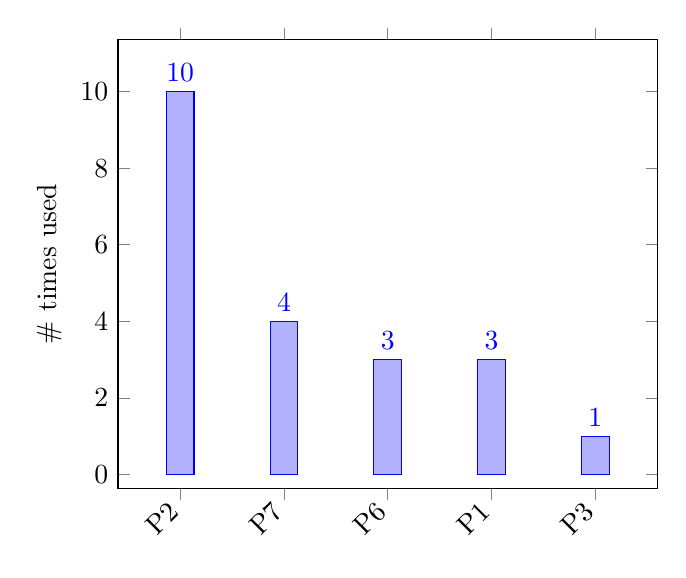
\begin{tikzpicture}
	  \begin{axis}[
	    ybar,
	    enlargelimits=0.15,
	    legend style={at={(0.5,-0.2)},
	      anchor=north,legend columns=-1},
	    ylabel={\# times used},
	    symbolic x coords={P2,P7,P6, P1,P3},
	    xtick=data,
	    nodes near coords, 
		nodes near coords align={vertical},
	    x tick label style={rotate=45,anchor=east},
	    ]
	    \addplot coordinates {(P2,10) (P7,4) 
			(P6,3) (P1,3) (P3,1)};
	  \end{axis}
	\end{tikzpicture}
	\label{fig:preprocess_usage}
	\caption[Statistics of pre-processing usage.]{Statistics of pre-processing usage. Removing all usernames, urls hash-tag character, RT-tag and excessive letters as features seem to perform the best.}
\end{figure}

\section{Experiment Results}
\textcolor{blue}{Show plots, significant features and so on and describe the results from the experiment}

\subsection{Grid Search}
As described above, an extensive grid search was conducted. This search cycled through different algorithms, parameters and preprocessing techniques. Figure~\ref{fig:results_full} displays the precision, recall, F-measure and accuracy for each of the classifiers with test set 1 as evaluation data. We notice that most of the classifiers that includes the NB algorithm has a bad performance, both for accuracy and F-measure. This was observed for other test sets as well. Further, we can see that the MaxEnt classifier has the best accuracy, while SVM has a slightly better F-measure.

We can also see that all the classifiers with SVM tends to give a better cofusion matrix than the others. This is showed in Figures (firstconf - lastconf).

\subsubsection{Parameters and options}
As a part of the grid search, the system tried to apply all the different preprocessing methods for each classifier. Figure~\ref{fig:preprocess_usage} clearly shows that P2 (removing user names, URLs, hash-tag prefixes, RT-tokens and redundant letters) is the preprocessing method that was used most often, i.e., it gave the best accuracy. Figure~\ref{fig:preprocess_usage} also indicates that URLs are noisy, and does not contain any sentiment, and that hash-tags and emoticons are valuable features.


Notes:
\begin{enumerate}
\item Grid search across params result in MaxEnt being the best. With following params:
	\begin{itemize}
		\item 'ngram\_range': (1,1),
		\item  'sublinear\_tf': True,
		\item  'preprocessor': P3,
		\item  'use\_idf': True,
		\item  'smooth\_idf': True,
		\item  'max\_df': 0.5,
		\item  'stop\_words': None
	\end{itemize}
	\begin{itemize}
		\item 'C': 1.0,
		\item 'penalty': 'l1'
	\end{itemize}
	
\item Best impl has a accuracy of 0.645, but a bad confusion matrix.

\item SVM also performs well (probably better). Best params:
	\begin{itemize}
		\item 'ngram\_range': (1,1),
		\item  'sublinear\_tf': True,
		\item  'preprocessor': P2,
		\item  'use\_idf': True,
		\item  'smooth\_idf': True,
		\item  'max\_df': 0.5,
		\item  'stop\_words': None
	\end{itemize}
	\begin{itemize}
		\item 'C': 0.3
	\end{itemize}

\item Best impl of SVM has a accuracy of 0.638, better confusion matrix than MaxEnt

\item Overall stats for feature filters:
	\begin{description}
		\item[remove\_noise] 10
		\item[no\_url\_usernames\_reduced\_attached] 4
		\item[placeholders] 1
		\item[reduced\_attached] 3
		\item[no\_usernames] 3
	\end{description}

\item SVM uses remove\_noise (P2) and MaxEnt is the only one using placeholders (P3). 
 
\item Can see that even though maxent scored better, it has a worse confusion matrix, than SVM. Not much difference in accuracy really. 

\item SVM and MaxEnt is performs much better than the rest. 
\end{enumerate}

Some other text... 

\begin{sidewaysfigure}[htb]
 \begin{center}
     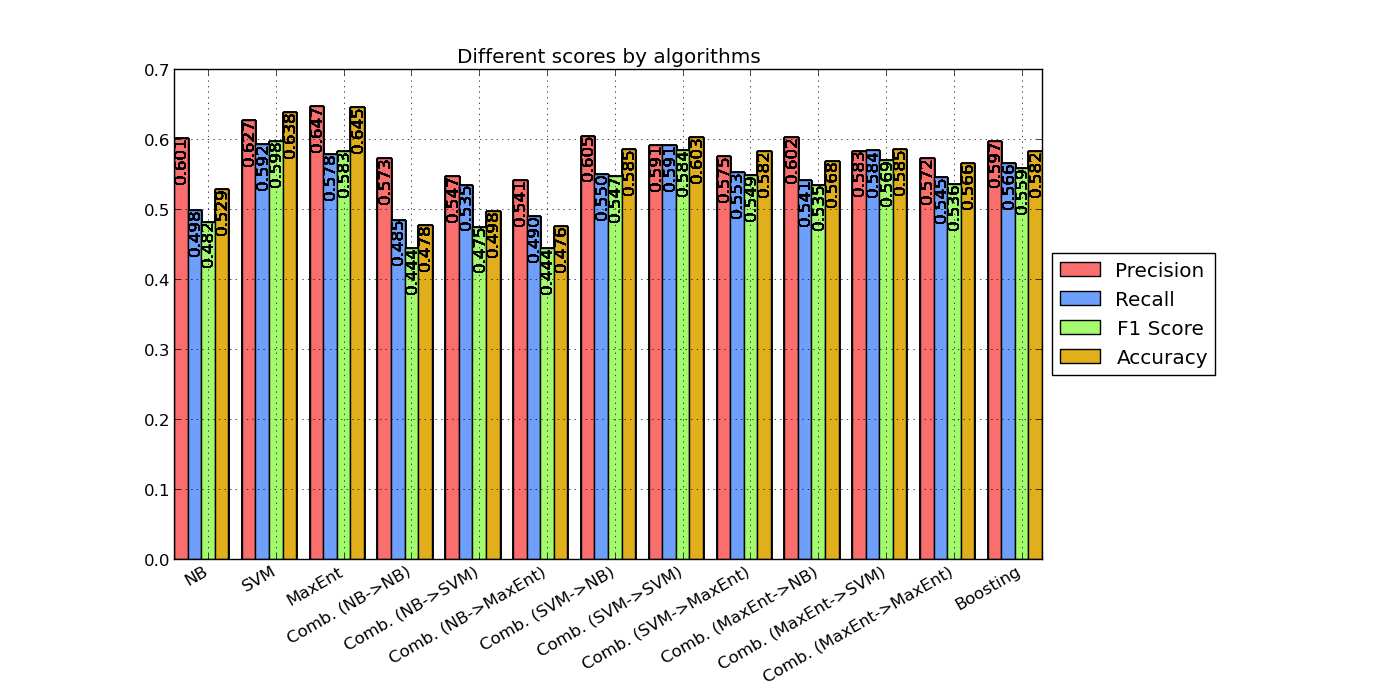
\includegraphics[width=\linewidth]{../img/plots/grid/full.png}
 \end{center}
 \caption[Results overview across models]{A full overview of the performance of the different models after a full grid search. Two models sticks out as having highest accuracies: SVM and MaxEnt. One can also see models using Naive Bayes, especially on it's own or to classify subjectivity, performs poorly.}
 \label{fig:results_full}
\end{sidewaysfigure}



\begin{minipage}[s]{\linewidth}
     \centering
     \begin{minipage}{0.45\linewidth}
          \begin{figure}[H]
               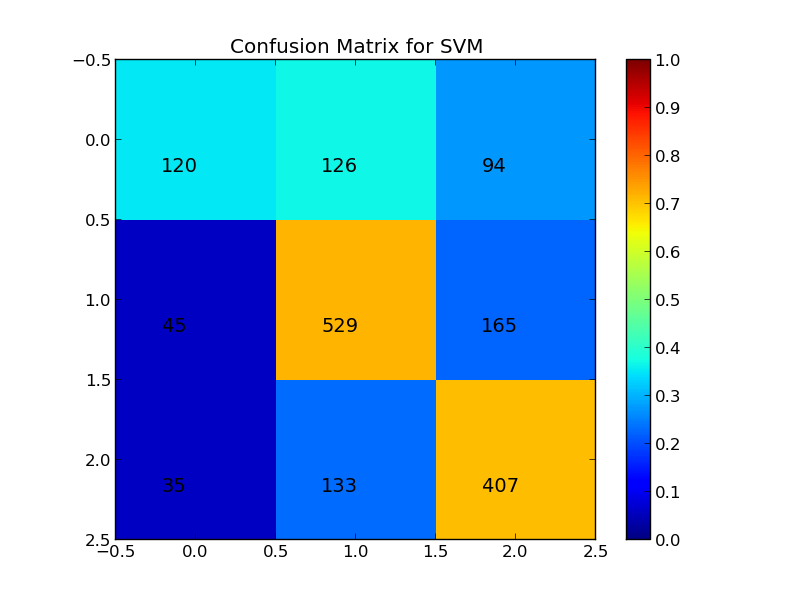
\includegraphics[width=\linewidth]{../img/plots/grid/confusion_matrix_SVM.png}
           \caption[Plot showing the confusion matrix for SVM]{Confusion matrix for the model using SVM. Performs well on both neutral and positive predictions, but somewhat poorer on negative.}
           \label{fig:confmat_svm}
          \end{figure}
     \end{minipage}
     \hspace{0.05\linewidth}
     \begin{minipage}{0.45\linewidth}
          \begin{figure}[H]
               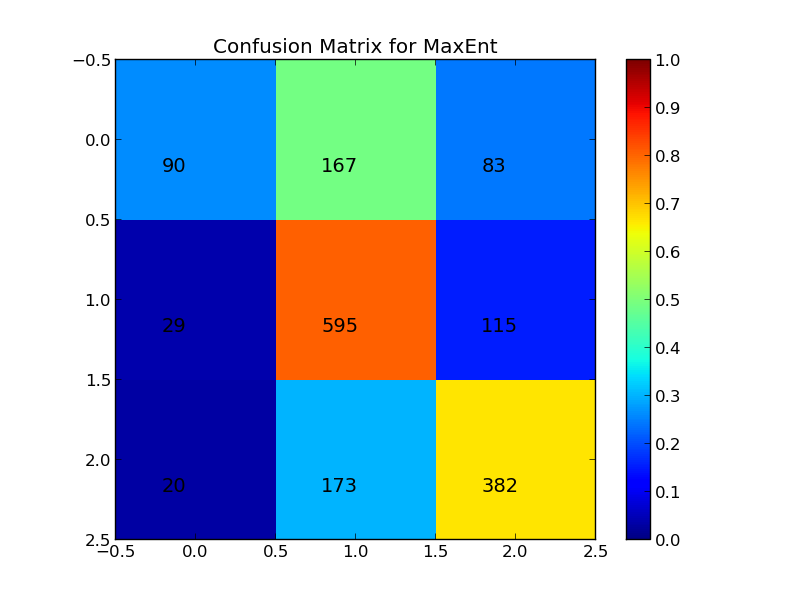
\includegraphics[width=\linewidth]{../img/plots/grid/confusion_matrix_MaxEnt.png}
           \caption[Plot showing the confusion matrix for MaxEnt]{Confusion matrix for the model using MaxEnt. Performs especially good on neutral tweets, but seem to be classifying neutral too much.}
           \label{fig:confmat_maxent}
          \end{figure}
     \end{minipage} \\
 
     \begin{minipage}{0.45\linewidth}
          \begin{figure}[H]
               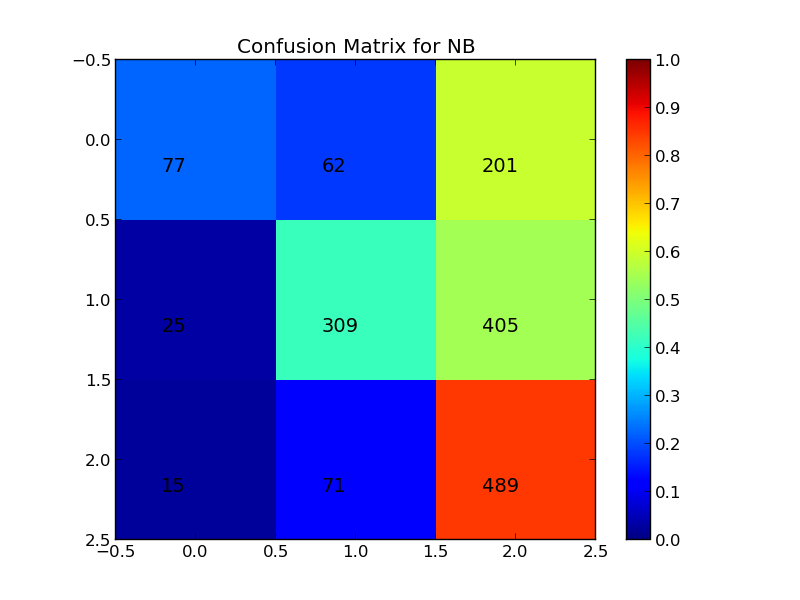
\includegraphics[width=\linewidth]{../img/plots/grid/confusion_matrix_NB.png}
           \caption[Plot showing the confusion matrix for NB]{Confusion matrix for the model using NB. Performs very well for positive tweets, but seem to favour it too much.}
           \label{fig:confmat_nb}
          \end{figure}
     \end{minipage}
     \hspace{0.05\linewidth}
     \begin{minipage}{0.45\linewidth}
          \begin{figure}[H]
               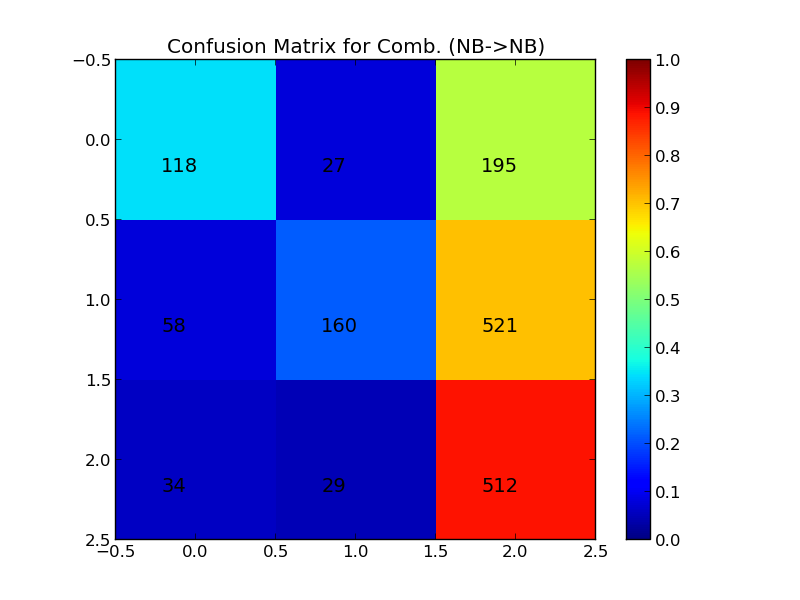
\includegraphics[width=\linewidth]{../img/plots/grid/confusion_matrix_Comb-NB-NB.png}
           \caption[Plot showing the confusion matrix for two-step NB -> NB]{Confusion matrix for the two-step model using NB for subjectivity/objectivity classification and NB for polarity. Shows the same trend as when using NB in a one-step model. Model favours positive predictions.}
           \label{fig:confmat_nb_nb}
          \end{figure}
     \end{minipage}   \\
         

     \begin{minipage}{0.45\linewidth}
          \begin{figure}[H]
               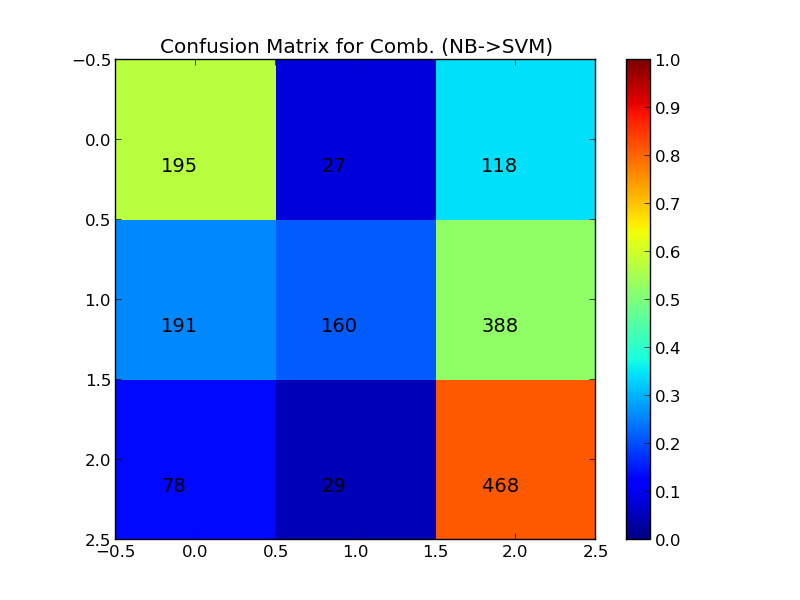
\includegraphics[width=\linewidth]{../img/plots/grid/confusion_matrix_Comb-NB-SVM.png}
           \caption[Plot showing the confusion matrix for two-step NB -> SVM]{Confusion matrix for the two-step model using NB for subjectivity/objectivity classification and SVM for polarity. Shows the same trend as when using NB in a one-step model. Model favours positive predictions but performing better for negative tweets.}
           \label{fig:confmat_nb_svm}
          \end{figure}
     \end{minipage}
     \hspace{0.05\linewidth}
     \begin{minipage}{0.45\linewidth}
          \begin{figure}[H]
               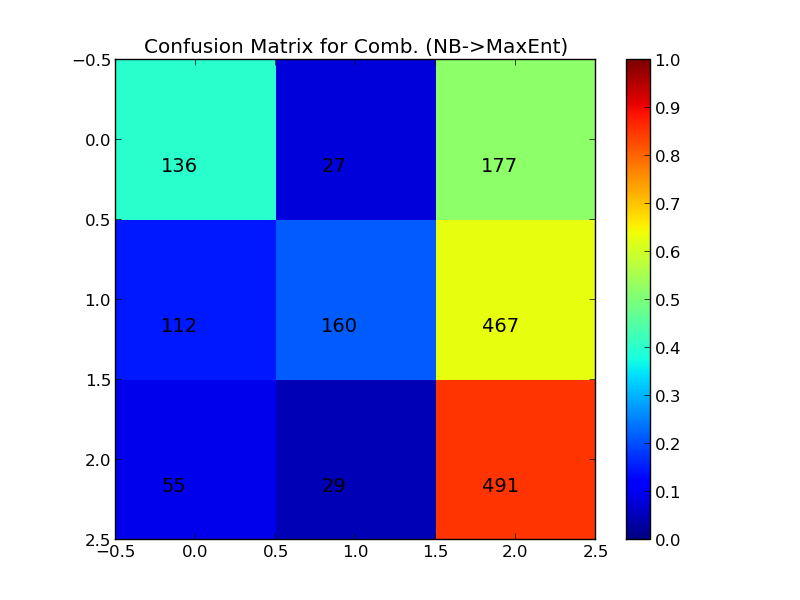
\includegraphics[width=\linewidth]{../img/plots/grid/confusion_matrix_Comb-NB-MaxEnt.png}
           \caption[Plot showing the confusion matrix for two-step NB -> MaxEnt]{Confusion matrix for the two-step model using NB for subjectivity/objectivity classification and SVM for polarity. Shows the same trend as when using the NB -> SVM model. Model favours positive predictions but performing better for negative tweets.}
           \label{fig:confmat_nb_maxent}
          \end{figure}
     \end{minipage}
\end{minipage}


\begin{minipage}[s]{\linewidth}
     \centering
     \begin{minipage}{0.45\linewidth}
           \begin{figure}[H]
                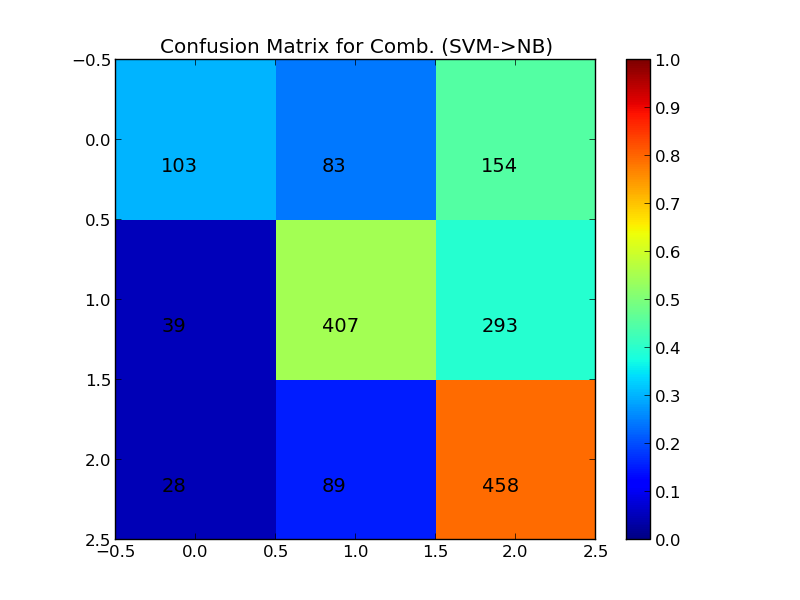
\includegraphics[width=\linewidth]{../img/plots/grid/confusion_matrix_Comb-SVM-NB.png}
         Plot showing the confusion matrix for two-step SVM -> NB]{Confusion matrix for the model using SVM and NB. Performs good for positive tweets, but not as good for neutral and negativion over here.}
            \label{fig:confmat_svm_nb}
           \end{figure}
      \end{minipage}
      \hspace{0.05\linewidth}
      \begin{minipage}{0.45\linewidth}
           \begin{figure}[H]
                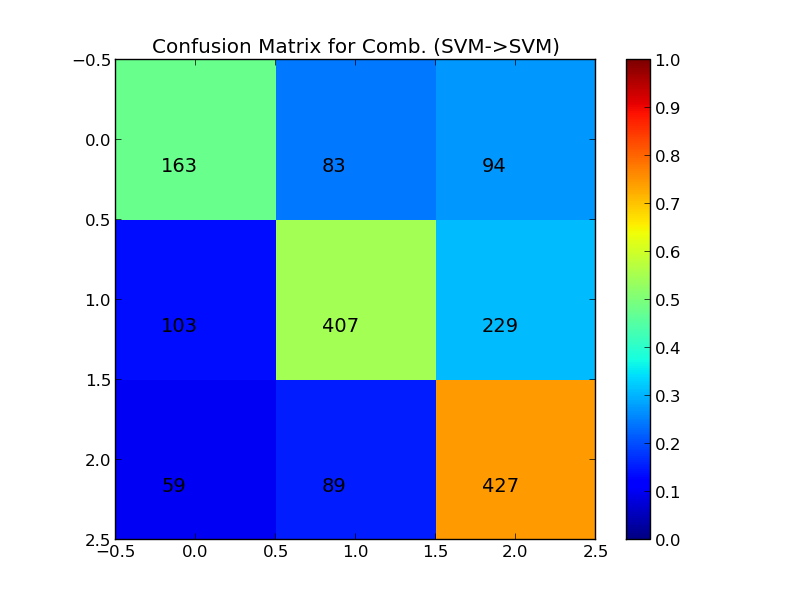
\includegraphics[width=\linewidth]{../img/plots/grid/confusion_matrix_Comb-SVM-SVM.png}
         Plot showing the confusion matrix for two-step SVM -> SVM]{Confusion matrix for the model using SVM and SVM. Performs good across the board, and shows a good diagonal colour profile in the ploton over here.}
            \label{fig:confmat_svm_svm}
           \end{figure}
      \end{minipage} \\
 
     \begin{minipage}{0.45\linewidth}
          \begin{figure}[H]
               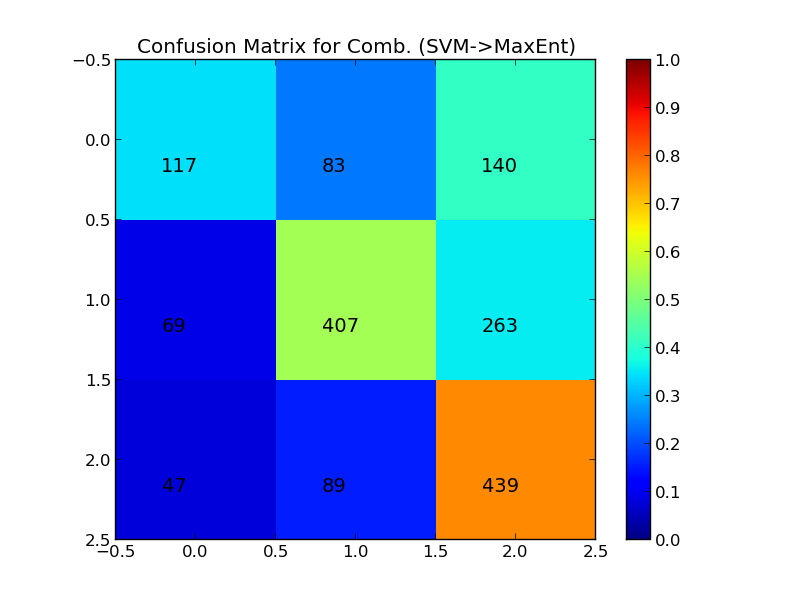
\includegraphics[width=\linewidth]{../img/plots/grid/confusion_matrix_Comb-SVM-MaxEnt.png}
           \caption[Plot showing the confusion matrix for two-step SVM -> MaxEnt]{Confusion matrix for the model using SVM and MaxEnt. Performs good for neutral and positive tweets, but not too well with negative tweets.}
           \label{fig:confmat_svm_maxent}
          \end{figure}
     \end{minipage}
     \hspace{0.05\linewidth}
     \begin{minipage}{0.45\linewidth}
          \begin{figure}[H]
               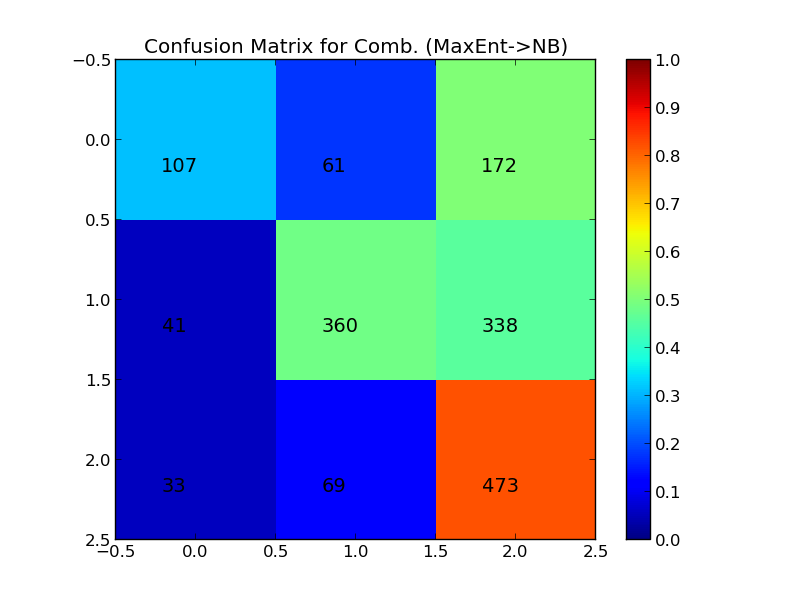
\includegraphics[width=\linewidth]{../img/plots/grid/confusion_matrix_Comb-MaxEnt-NB.png}
           \caption[Plot showing the confusion matrix for two-step MaxEnt -> NB]{Confusion matrix for the model using MaxEnt and NB. Performs good for positive tweets, but not too well with negative and neutral tweets.}
           \label{fig:confmat_maxent_nb}
          \end{figure}
     \end{minipage}   \\
         

     \begin{minipage}{0.45\linewidth}
          \begin{figure}[H]
               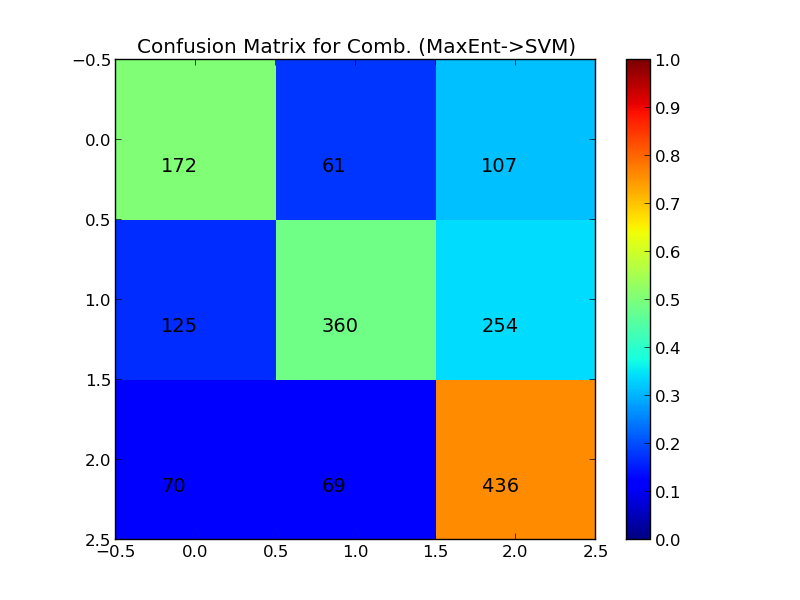
\includegraphics[width=\linewidth]{../img/plots/grid/confusion_matrix_Comb-MaxEnt-SVM.png}
           \caption[Plot showing the confusion matrix for two-step MaxEnt -> SVM]{Confusion matrix for the model using MaxEnt and SVM. Performs good but is too heavy on the positive classification.}
           \label{fig:confmat_maxent_svm}
          \end{figure}
     \end{minipage}
     \hspace{0.05\linewidth}
     \begin{minipage}{0.45\linewidth}
          \begin{figure}[H]
               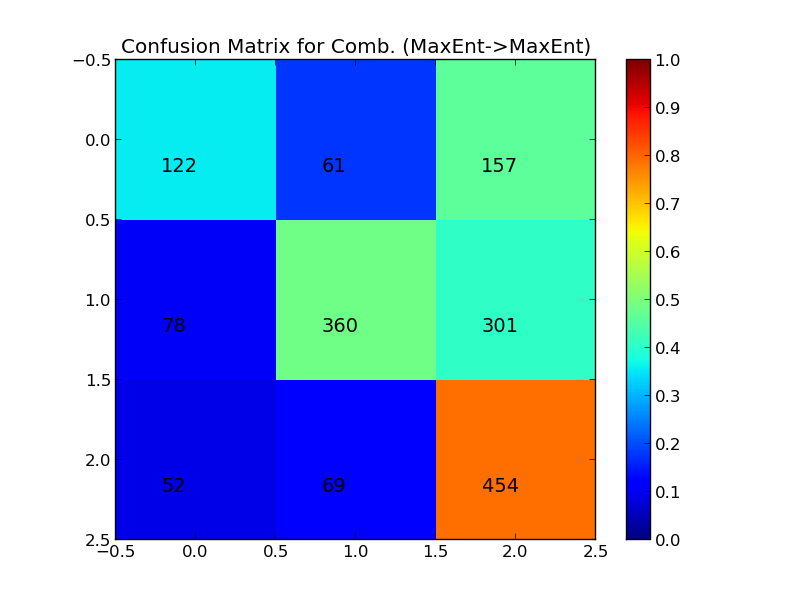
\includegraphics[width=\linewidth]{../img/plots/grid/confusion_matrix_Comb-MaxEnt-MaxEnt.png}
           \caption[Results overview across models]{Caption description over here.}
           \label{fig:confmat_maxent_maxent}
          \end{figure}
     \end{minipage}
\end{minipage}

\begin{figure}[H]
 \begin{center}
     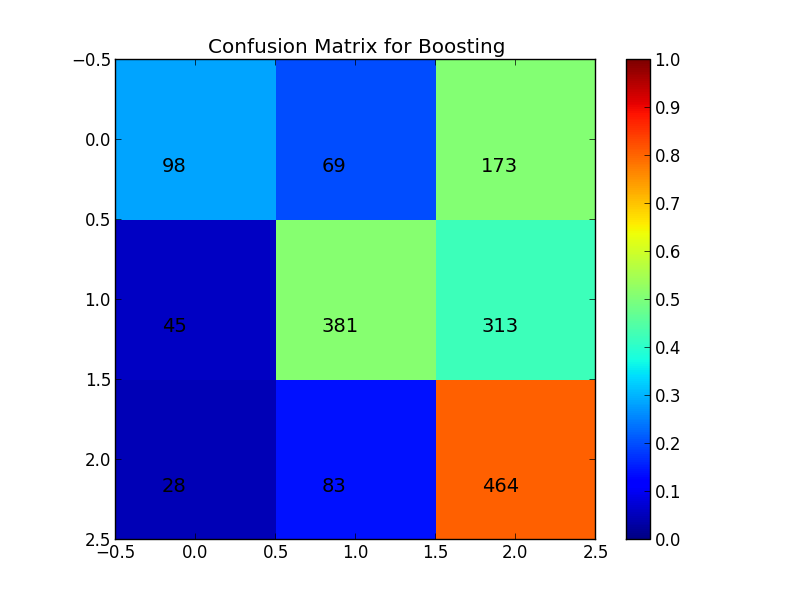
\includegraphics[width=0.7\linewidth]{../img/plots/grid/confusion_matrix_Boosting.png}
 \end{center}
 \caption[Results overview across models]{Caption description over here.}
 \label{fig:confmat_boosting}
\end{figure}


\begin{table}[htb]
\centering
\begin{tabular}{|r||c|c|c|} 
\cline{2-3}
\multicolumn{1}{c|}{ } & \textbf{SVM} & \textbf{MaxEnt} \\ \hline
ngram\_range & 1,1 & 1,1 \\ \hline
sunlinear\_tf  & True & True \\ \hline
preprocessor & P2 & P3 \\ \hline
use\_idf & True & True \\ \hline
smooth\_idf & True & True \\ \hline
max\_df & 0.5 & 0.5 \\ \hline
stop\_words & None & None \\ \hline
C & 1.0 & 0.3 \\ \hline
penalty & l1 & \\ \hline

\end{tabular}
\caption{Best parameters for SVM and MaxEnt.}
\label{tab:svm_maxent_best_params}
\end{table}



\begin{table}[!htb]
	
	\begin{minipage}{.45\linewidth}
		\begin{tabular}{|c|c|c|}
		
		\multicolumn{3}{c}{SVM} \\ \hline
		
		Negative & Neutral & Positive \\ \hline\hline
		
		no  		& wear & wait \\ \hline
		didn't  	& tallahassee & nice \\ \hline
		cancelled  	& 15th & interesting \\ \hline
		don't  		& 26 & awesome \\ \hline
		worse  		& at & cool \\ \hline
		why  		& trip & amazing \\ \hline
		bad  		& joe & fun \\ \hline
		worst  		& theres & ! \\ \hline
		hate  		& arrows & :) \\ \hline
		shit  		& murphy, & excited \\ \hline
		sad  		& question & happy \\ \hline
		sorry  		& plan & love \\ \hline
		not  		& set & best \\ \hline
		fuck  		& 8th & great \\ \hline
		:(  		& paterno & good \\ \hline
		\end{tabular}
	\end{minipage}
	\hspace{0.05\linewidth}
	\begin{minipage}{.45\linewidth}
		\begin{tabular}{|c|c|c|}

		
		\multicolumn{3}{c}{MaxEnt} \\ \hline
		
		Negative & Neutral & Positive \\ \hline\hline
		
		no 	& center & glad \\ \hline
		don't 	& royal & nice \\ \hline
		why 	& plan & thanks \\ \hline
		bad 	& joe & cool \\ \hline
		shit 	& nov & awesome \\ \hline
		injury 	& george & interesting \\ \hline
		cancelled 	& theres & amazing \\ \hline
		hate 	& arrows & :) \\ \hline
		worst 	& trip & fun \\ \hline
		worse 	& set & best \\ \hline
		fuck 	& question & excited \\ \hline
		sorry 	& at & love \\ \hline
		not 	& url & happy \\ \hline
		sad 	& 8th & good \\ \hline
		:( 	& paterno & great \\ \hline
		\end{tabular}
	\end{minipage}
	\caption[Most informative features]{Top 15 of the most informative features for SVM and MaxEnt}
	\label{tab:informative_features}
\end{table}



\section{NOTE: Analysis part: SVM vs MaxEnt}

\begin{figure}[htb]
	\centering
	\begin{minipage}{.45\linewidth}
		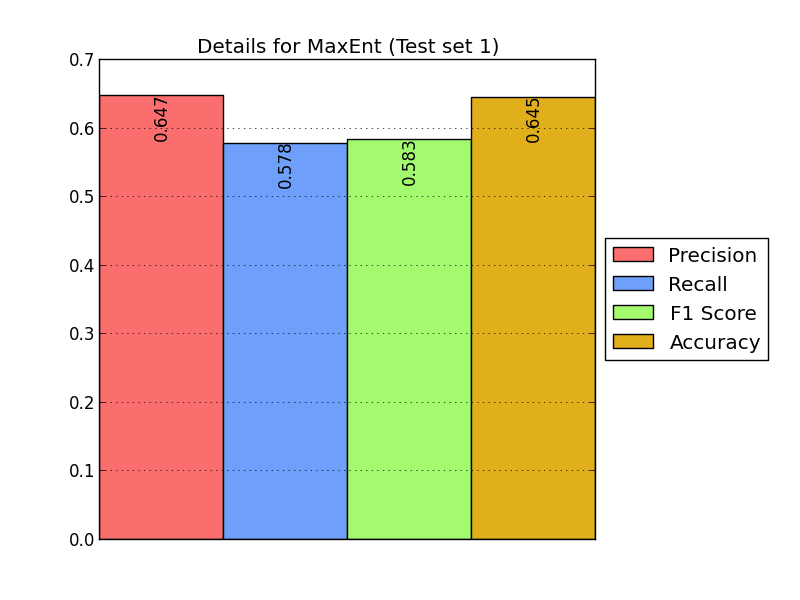
\includegraphics[width=\linewidth]{../img/plots/analysis/maxent_stats_best.png}
	\end{minipage}
	\hspace{0.05\linewidth}
	\begin{minipage}{.45\linewidth}
		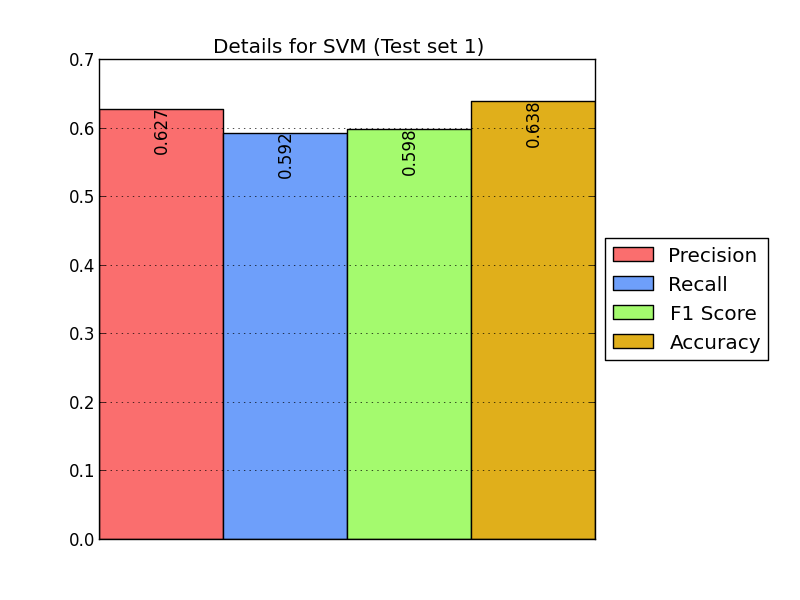
\includegraphics[width=\linewidth]{../img/plots/analysis/svm_stats_best.png}
	\end{minipage}
	\caption[Best performance plots for SVM and MaxEnt]{Best performance plots for SVM and MaxEnt}
	\label{fig:best_result}
\end{figure}

\begin{figure}[htb]
	\centering
	\begin{minipage}{.45\linewidth}
		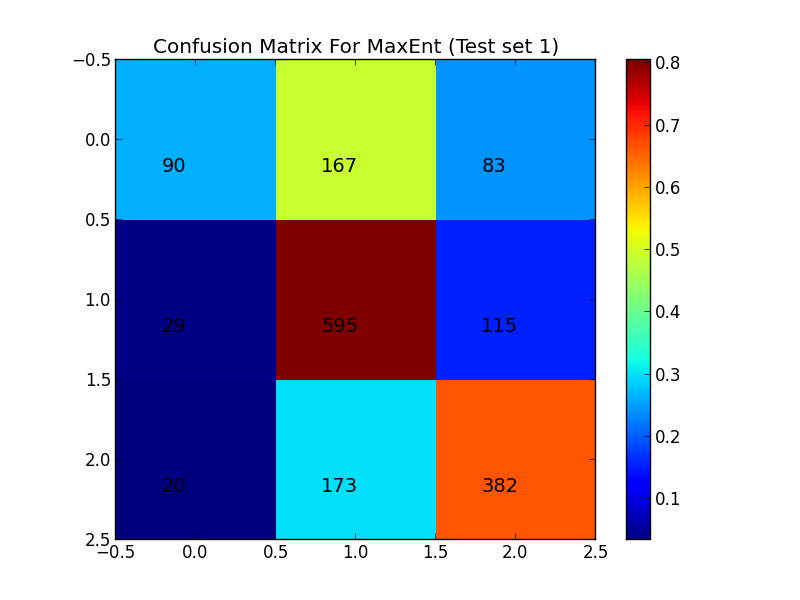
\includegraphics[width=\linewidth]{../img/plots/analysis/maxent_confusion_matrix_best.png}
	\end{minipage}
	\hspace{0.05\linewidth}
	\begin{minipage}{.45\linewidth}
		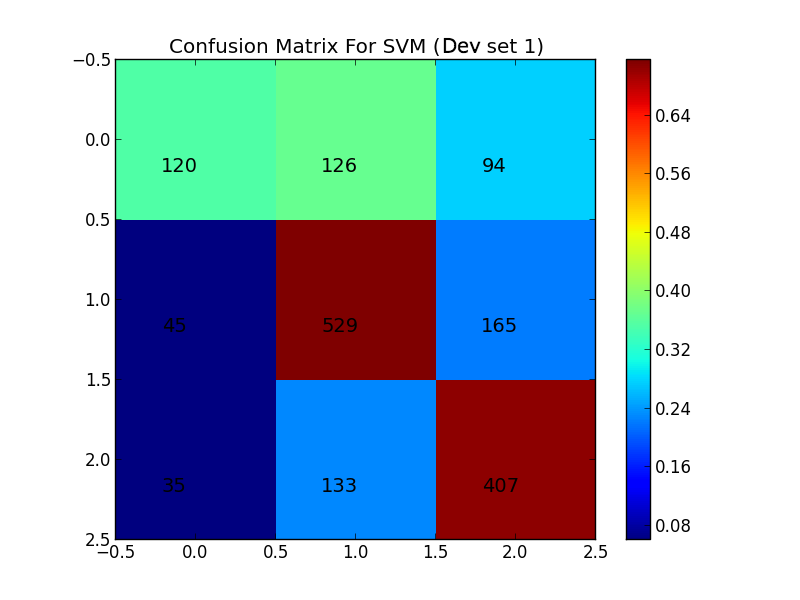
\includegraphics[width=\linewidth]{../img/plots/analysis/svm_confusion_matrix_best.png}
	\end{minipage}
	\label{fig:best_result_confusion}
	\caption[Confusion Matrix for SVM and MaxEnt]{Confusion Matrix for SVM and MaxEnt]}
\end{figure}





\begin{figure}[htb]
	\centering
	\begin{minipage}{.45\linewidth}
		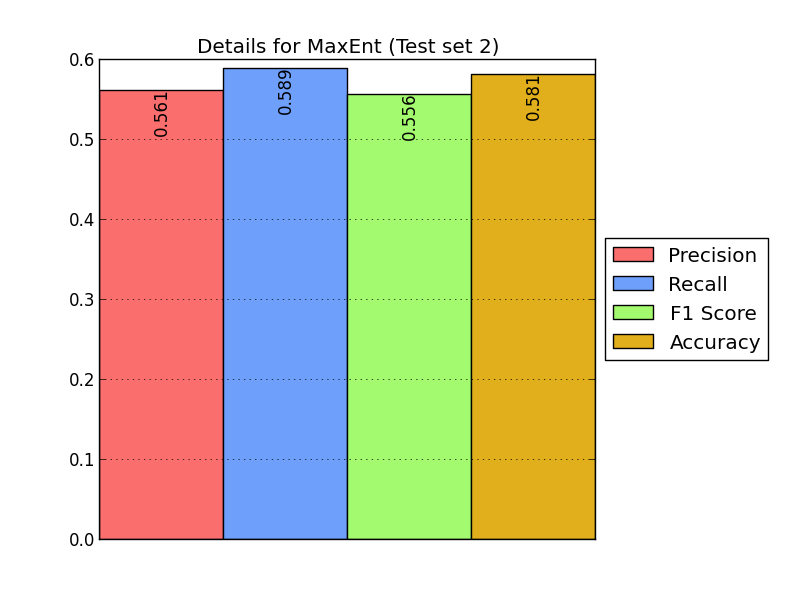
\includegraphics[width=\linewidth]{../img/plots/analysis/maxent_stats_best_diff_test.png}
	\end{minipage}
	\hspace{0.05\linewidth}
	\begin{minipage}{.45\linewidth}
		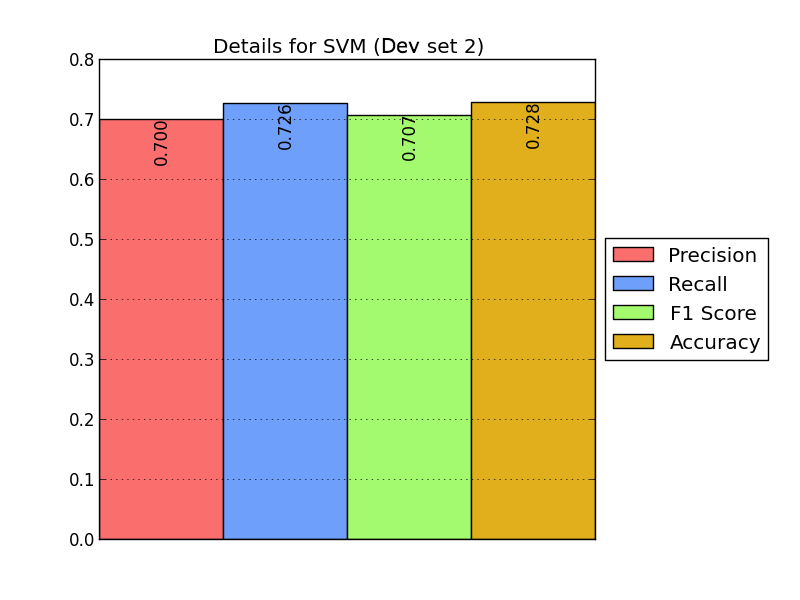
\includegraphics[width=\linewidth]{../img/plots/analysis/svm_stats_best_diff_test.png}
	\end{minipage}
	\label{fig:best_result_testset2}
	\caption[Best performance plots for SVM and MaxEnt for test set 2]{Best performance plots for SVM and MaxEnt using test set 2}
\end{figure}

\begin{figure}[htb]
	\centering
	\begin{minipage}{.45\linewidth}
		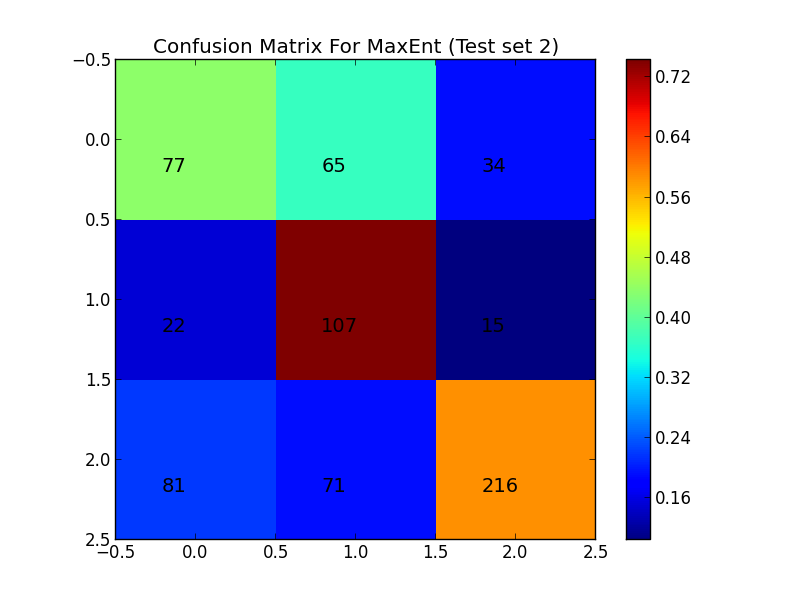
\includegraphics[width=\linewidth]{../img/plots/analysis/maxent_confusion_matrix_best_diff_test.png}
	\end{minipage}
	\hspace{0.05\linewidth}
	\begin{minipage}{.45\linewidth}
		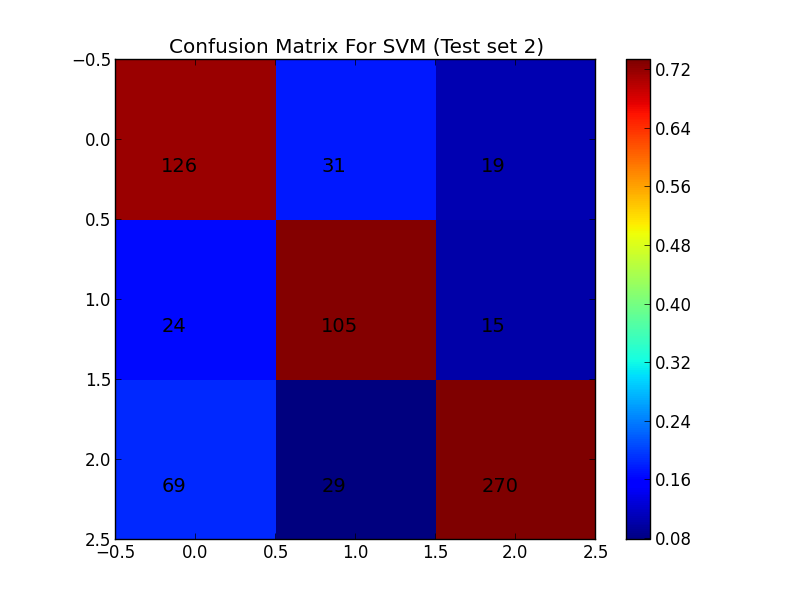
\includegraphics[width=\linewidth]{../img/plots/analysis/svm_confusion_matrix_best_diff_test.png}
	\end{minipage}
	\label{fig:best_result_confusion_testset2}
	\caption[Confusion Matrix for SVM and MaxEnt using test set 2]{Confusion Matrix for SVM and MaxEnt using test set 2}
\end{figure}



\begin{figure}[htb]
	\centering
	\begin{minipage}{.45\linewidth}
		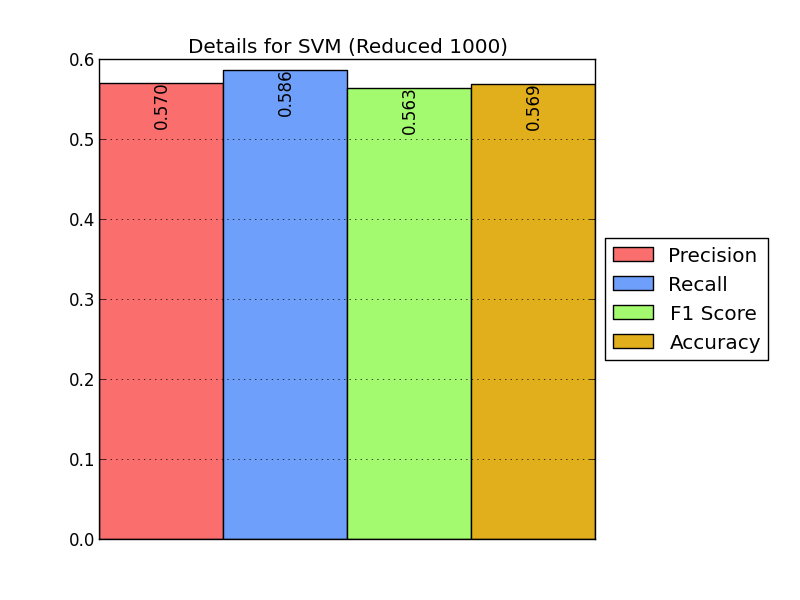
\includegraphics[width=\linewidth]{../img/plots/analysis/svm_stats_best_reduced_1000.png}
	\end{minipage}
	\hspace{0.05\linewidth}
	\begin{minipage}{.45\linewidth}
		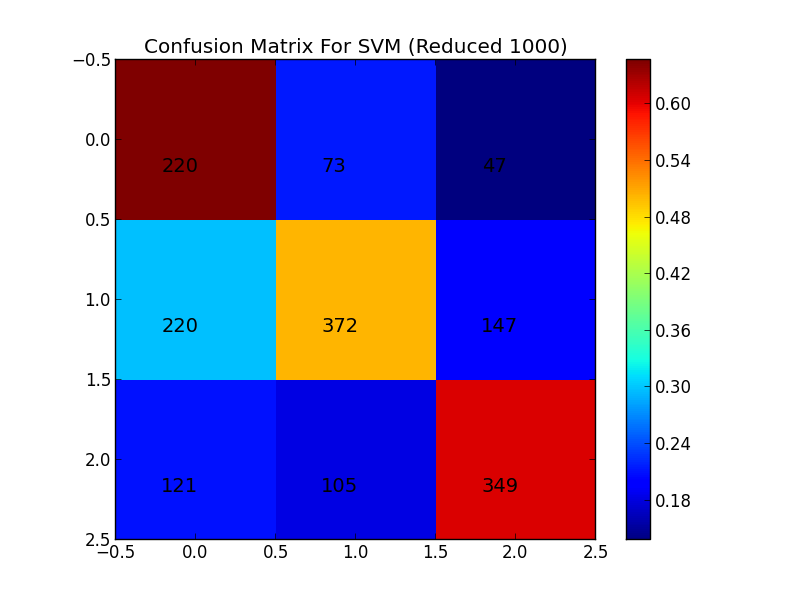
\includegraphics[width=\linewidth]{../img/plots/analysis/svm_confusion_matrix_best_reduced_1000.png}
	\end{minipage}
	\label{fig:svm_reduced_1000}
	\caption[Performance of SVM when reduced dataset to max 1000 per class]{Performance of SVM when reduced dataset to max 1000 per class}
\end{figure}

\begin{figure}[htb]
	\centering
	\begin{minipage}{.45\linewidth}
		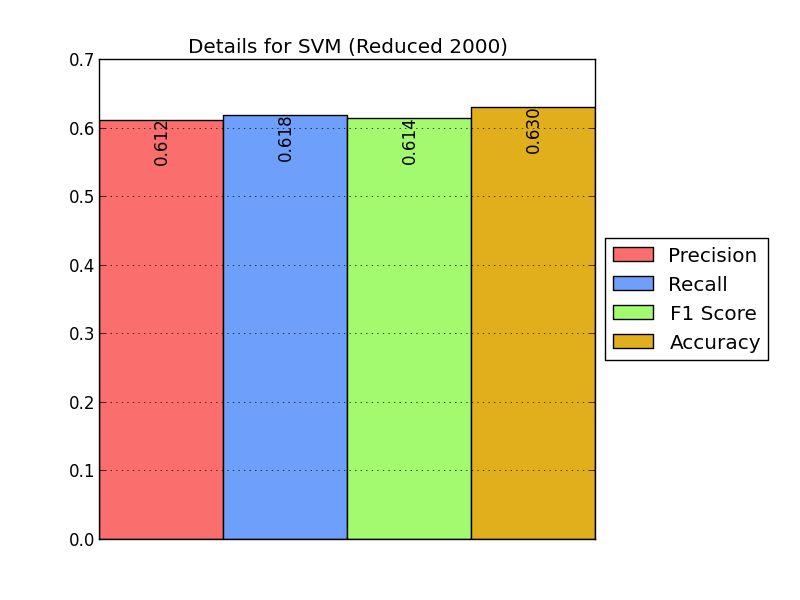
\includegraphics[width=\linewidth]{../img/plots/analysis/svm_stats_best_reduced_2000.png}
	\end{minipage}
	\hspace{0.05\linewidth}
	\begin{minipage}{.45\linewidth}
		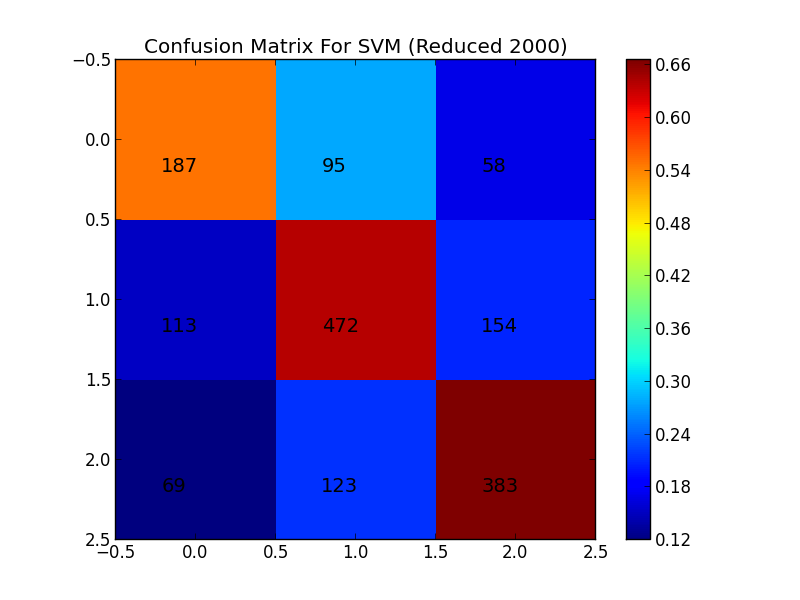
\includegraphics[width=\linewidth]{../img/plots/analysis/svm_confusion_matrix_best_reduced_2000.png}
	\end{minipage}
	\label{fig:svm_reduced_2000}
	\caption[Performance of SVM when reduced dataset to max 2000 per class]{Performance of SVM when reduced dataset to max 1000 per class}
\end{figure}
